\documentclass[sigconf]{acmart}

\usepackage{booktabs} % For formal tables
\usepackage{minted}
\usepackage{graphicx}
\usepackage{tabularx}
\usepackage{arydshln}
\usepackage{subcaption}
%\usepackage{times}
\usepackage{hyperref}
\usepackage{array}
\usepackage[normalem]{ulem}
%\hypersetup{
%    colorlinks=true,
%    linkcolor=blue,
%    filecolor=magenta,      
%    urlcolor=cyan,
%}
%\setlength{\belowcaptionskip}{-5pt}




% Copyright
%\setcopyright{none}
%\setcopyright{acmcopyright}
%\setcopyright{acmlicensed}
\setcopyright{rightsretained}
%\setcopyright{usgov}
%\setcopyright{usgovmixed}
%\setcopyright{cagov}
%\setcopyright{cagovmixed}


\begin{document}
\title{Popper Pitfalls: Experiences Following \\a Reproducibility Convention}

\author{Michael A. Sevilla}
\affiliation{%
 \institution{University of California, Santa Cruz}}
\email{msevilla@soe.ucsc.edu}

\author{Carlos Maltzahn}
\affiliation{%
  \institution{University of California, Santa Cruz}}
\email{carlosm@ucsc.edu}

\begin{abstract}

We describe the four publications we have tried to make reproducible and
discuss how each paper has changed our workflows, practices, and collaboration
policies. The fundamental insight is that paper artifacts must be made
reproducible from the start of the project; artifacts are too difficult to make
reproducible when the papers are (1) already published and (2) authored by
researchers that are not thinking about reproducibility. In this paper, we
present the best practices adopted by our research laboratory, which was
sculpted by the pitfalls we have identified for the Popper convention.  We
conclude with a ``call-to-arms" for the community focused on enhancing
reproducibility initiatives for academic conferences, industry environments,
and national laboratories. We hope that our experiences will shape a best
practices guide for future reproducible papers.

\end{abstract}



%
% The code below should be generated by the tool at
% http://dl.acm.org/ccs.cfm
% Please copy and paste the code instead of the example below.
%
\begin{CCSXML}
<ccs2012>
<concept>
<concept_id>10011007.10011074.10011092.10011096</concept_id>
<concept_desc>Software and its engineering~Reusability</concept_desc>
<concept_significance>500</concept_significance>
</concept>
<concept>
<concept_id>10011007.10011074.10011099.10011693</concept_id>
<concept_desc>Software and its engineering~Empirical software validation</concept_desc>
<concept_significance>500</concept_significance>
</concept>
<concept>
<concept_id>10011007.10011074.10011111.10011113</concept_id>
<concept_desc>Software and its engineering~Software evolution</concept_desc>
<concept_significance>300</concept_significance>
</concept>
<concept>
<concept_id>10011007.10011074.10011134</concept_id>
<concept_desc>Software and its engineering~Collaboration in software development</concept_desc>
<concept_significance>100</concept_significance>
</concept>
</ccs2012>
\end{CCSXML}

\ccsdesc[500]{Software and its engineering~Reusability}
\ccsdesc[500]{Software and its engineering~Empirical software validation}
\ccsdesc[300]{Software and its engineering~Software evolution}
\ccsdesc[100]{Software and its engineering~Collaboration in software development}
\keywords{Software Testing ; Performance Engineering}

\copyrightyear{2018} 
\acmYear{2018} 
\setcopyright{acmcopyright}
\acmConference[P-RECS'18]{First International Workshop on Practical Reproducible Evaluation of Computer Systems}{June 11, 2018}{Tempe, AZ, USA}
\acmBooktitle{P-RECS'18: First International Workshop on Practical Reproducible Evaluation of Computer Systems, June 11, 2018, Tempe, AZ, USA}
\acmPrice{15.00}
\acmDOI{10.1145/3214239.3214243}
\acmISBN{978-1-4503-5861-3/18/06}

\maketitle

\section{Introduction}

\section{Popper-compliant Papers}

% what papers have we done
We have authored five Popper-compliant papers:
\begin{itemize}

\item quiho: Automated Performance Regression Testing Using Inferred
Resource Utilization Profiles

\item Cudele: An API and Framework for Programmable Consistency and
Durability in a Global Namespace

\item Malacology: A Programmable Storage System

\item Characterizing and Reducing Cross-Platform Performance Using
OS-level Virtualization

\item Programmable Caches with a Data Management Language \& Policy Engine

\end{itemize}

Popper 


\section{Reproducibility Must Be a 1st Class Citizen}
% exploration vs. complete
% cross-cluster compatibility 
%  - inventory files hard coded throughout tree
%  - configuration files not propagated for experiments
%  - visualize files pulled data from hard coded paths
%  - graphs not created automatically
% why Mantle failed

\section{Organized Repositories and Documentation}
%cause the most work
% role of git
% docker images saved in internal registry (buildding)

\section{Well-Defined Collaboration Roles}
% keeping organization
% workflows

\section{Maintaining Pointers}
% wary of ephemeral links

% large code bases large code bases (src, deploy)

% different registry hubs (Docker, GitHub)

\section{Conference Requirements}
% double blinded??

\section{Conclusion}

\section{Popper-compliant Papers}
\label{sec:popper-compliant-papers}

We have produced four Popper-compliant papers, as shown in
Table~\ref{table:papers}. These papers follow the reader/reviewer sample
workflow outlined in~\cite{jimenez:ipdpsw17-popper} and shown in
Figure~\ref{fig:workflow}. For the visualization component (1), we use Jupyter
notebooks. The notebooks themselves are versioned with Git and users interact
with local copies by cloning the repository and launching a Jupyter Docker
container. The paper is written in \LaTeX and built with a Docker container.
For the code component (2), both the source code for the system itself and the
deploy/experiment code is stored on GitHub. When running experiments, we use
Docker containers to isolate libraries and binaries. For the multi-node
component (3), we use CloudLab machines and Ansible to script deployment and
experiment orchestration. For the data set components (4), we use GitHub to
store results files; our inputs and results are small enough that we do no need
a larger capacity.  GitHub allows files up to 50MB and stores data on S3.

Our experiments start with a baseline. To describe the process, we reference
our
ceph-popper-template\footnote{https://github.com/michaelsevilla/ceph-popper-template}
set up on CloudLab. Users setup SSH keys and deploy CloudLab nodes using our
CephFS Profile\footnote{https://www.cloudlab.us/p/CephFS/CephFS-HEP}.  The
profile has the nodes automatically install Docker on bootup using our
install\footnote{https://github.com/michaelsevilla/ceph-popper-template/blob/master/hardware/cloudlab/\-install.sh}
script. After the nodes finish booting ({\it i.e.}  their status on the
CloudLab GUI is READY), users push SSH keys using a convenience
script\footnote{https://raw.githubusercontent.com/michaelsevilla/ceph-popper-template/master/hardware/cloudlab/pushkeys.sh}.

The deploy code is based on
ceph-ansible\footnote{https://github.com/ceph/ceph-ansible/wiki}, a tool that
configures hardware and software for Ceph. We forked the project and made it
less dependent on Python. To run an experiment, users log into the head node
and clone the ceph-popper-template repository. This repository has submodules
that point to ceph-ansible and our own custom roles; configuration files for
our Ceph setup; and helper scripts written in bash that deploy Ceph and run the
benchmarks.  For more information on the Ceph template, see the
README\footnote{https://github.com/michaelsevilla/ceph-popper-template} and for
more information on the baseline and pipelines terminology, see the Popper
Convention quickstart\footnote{http://falsifiable.us/}. 

\begin{figure}[tb] 
  \centering
  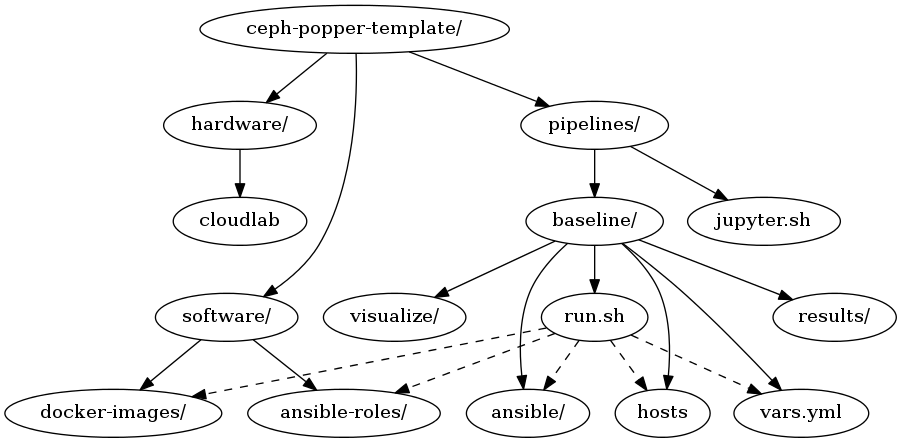
\includegraphics[width=1\linewidth]{./figures/expdir.png}
  \caption{Organization of our experiment directories. \texttt{baseline/} is an
example experiment and contains scripts populated with the Popper CLI. The
\texttt{run.sh} script uses many directories and files to setup and run
experiments, as indicated by the dashed lines.}
  \label{fig:expdir}
\end{figure}

An outline of this organization is shown in Figure~\ref{fig:expdir}, where
solid lines are directory links and dashed lines indicate which directories a
script uses.  A sample experiment is in the \texttt{baseline/} directoriy,
which was created using the Popper CLI. Users configure their cluster by
specifying hostnames and login user names in the \texttt{hosts} file.  Users
also specify the Ceph services that should be deployed using the
\texttt{ansible/}
directory\footnote{https://github.com/michaelsevilla/ceph-popper-template/tree/master/pipelines/baseline/ansible}.
This directory has code for deploying Ceph and its components, where the
\texttt{*.yml} files are Ansible playbooks that start and configure components:
\texttt{ceph.yml} starts Ceph and can be modified to specify which daemons to
launch, \texttt{cleanup.yml} tears Ceph down, and \texttt{monitor.yml} starts
daemons that monitor performance.  High level configurations are in the
\texttt{vars.yml} file.  We separate these components into different playbooks
so users can mix and match Ceph services.  Similarly, the workloads directory
has scripts for running the baseline benchmarks. The other files and
directories are Ansible configuration files used by the playbooks. We have
posted a tutorial on our
blog\footnote{http://programmability.us/mantle/blog2-ceph} to guide users
through this setup. When complete, users execute the \texttt{run.sh} to start
the job.



\section{Popper Pitfalls}
\label{popper-best-practices}

To produce Popper-compliant papers, we needed to change our workflows and
experimental procedures. We have shaped our best practices from the following pitfalls:

\subsection{Reproducibility is not a 1st Class Citizen}
\label{sec:repro}

% exploration vs. complete
Popper-compliance must be observed {\it throughout} the paper-writing process.
Attempts to make published papers Popper-compliant failed for three reasons:
(1) there is no incentive from the perspective of a researcher, (2) it is too
hard to remember the experimental workflow, and (3) the artifacts cannot be
added to the camera-ready article. We started trying to
make~\cite{sevilla:sc15-mantle}
Popper-compliant\footnote{https://github.com/michaelsevilla/mds} but gave up
because the effort would not have been rewarded, as the paper had already been
presented and published.

Making reproducibility a 1st class citizen introduces a careful design
decision: how does the user decide which results are exploratory and which are
complete. We do not want to waste space by saving results that do not
contribute to the paper but, at the same time, how do we know when an
experiment is worthy of being included in the paper? Discipline must be
exercised throughout the paper-writing process to make any experiment that is
deemed useful be immediately polished to be Popper-compliant.

% cross-cluster compatibility 
Another pitfall we face is cross-cluster compatibility. After identifying
results as being useful, we usually find cluster-specific files hard-coded
throughout the tree, configuration files randomly propagated to different
directories, visualization files reliant on data specified with hard-coded
paths, and graphs that are not created automatically. To address this, we must
exercise discipline to separate cluster-specific files from cluster-agnostic
files; we do this with \texttt{configs\_*/} directories in our
ceph-popper-template repository.

% organized repos/docs
Finally, organization and documentation must be required throughout the
paper-writing process. We failed to do this in early papers and this causes the
most work later on. System and experiment deploy code is rarely
self-explanatory. At a minimum, each experiment directory must contain a README
specifying how to run the jobs. To address this, we recommend relying heavily
on DockerHub, GitHub, and collaboration; making things public incentivizes 
tidiness and organization. Using internal Docker or Git repositories hampers
Popper-compliance and discourages community involvement.

\subsection{Poorly-Defined Collaboration Roles}

% keeping organization workflows
Collaboration  speeds up code development and, as stated in the previous
section, can be used as motivation to keeping Popper-compliant repositories;
but collaboration can also hamper the process.  Researchers have different
workflows and preferences. Committing system and experimental deploy code with
different toolkits, documentation, and styles to the same repository can result
in a confusing organizational structure.  To address this, we recommend that
the first author of the paper (1) produce a style guide, either by committing a
couple of experiments or adding detailed READMEs and (2) act as the gatekeeper
for all code. We recommend using GitHub because it nicely formats READMEs and
supports pull requests, issue trackers, and project boards.  Rather than having
meetings to agree on experiment organization, we recommend iteratively
combining code from collaborators with pull requests so the repository grows
organically and quickly in the style approved by the first author.

% merge conflicts
Another obstacle to collaboration is merge conflicts, especially when editing
the paper. We used to assign locks to people in an {\it ad-hoc} fashion over
email but this is not scalable. Instead, we now use Git to manage conflicts.
Before issuing a pull request, which notifies the first author, GitHub will
notify committers of changes they made in parallel with other changes. Our
policy is to force committers to resolve these merge conflicts before bothering
the first author. While we still recommend issuing pull requests to make sure
the first author approves of the style, the merge conflict workflow has been an
effective way to avoid annoying the first author with destructive changes.

\subsection{Failure to Maintain Pointers}

Popper-compliant papers provide pointers to graph artifacts, including results,
input files, and deploy code. But these links are problematic because they must
be maintained over time, even years after the paper is published. We have had
trouble maintaining these pointers because they (1) are ephemeral, (2) include
pointers to other repositories, and (3) include pointers to different
repository hosting sites.

%wary of ephemeral links
Ephemeral links and making sure that pointers are live is our biggest pain
point. Small, seemingly benign changes end up confusing users wanting to
reproduce our results. This is an artifact of how the internet was built, but
making sure that these links are live is one of the hardest challenges for
Popper-compliance. To combat this, we suggest maintaining continuous
integration pipelines that read the paper source code and send REST requests to
websites to ensure that 404 codes are not returned.

%large code bases large code bases (src, deploy)
Pointers to other repositories can make the Popper-compliant repository
confusing and difficult to navigate. For example, our Cudele paper had Git
submodule pointers to 3 other GitHub repositories: one for Ansible deployment
code for Ceph, one for Ansible deployment code for monitoring code written by
our research lab, and one for our paper bibliography. Users unfamiliar with
Ansible or \LaTeX would have trouble navigating these large code bases.
Unfortunately, this practice is necessary to avoid duplicating functionality
and ensuring future-proof modules. Our recommendation for addressing this
problem is to minimize the number of repository pointers and to document them
thoroughly, including the reasons that the pointer is necessary and what the
other repository does.

%different registry hubs (Docker, GitHub)
Finally, pointers to different repository sites can make Popper-compliant
papers difficult to understand. Again, this is a necessary evil because
research systems can be large and complicated with many moving parts. For
example, our Cudele paper uses a GitHub repository to maintain our source code
for our modified Ceph version, a GitHub repository to maintain our paper and
deploy code, a GitHub repository to maintain our common deploy code modules
(for monitoring), a DockerHub repository for housing software images with
compiled binaries for our modified Ceph version, and a CloudLab repository to
house our base images. Again, the recommended solution for maintaining this
complicated web of registry hubs is to thoroughly document the process.

%\subsection{Baselines}
% can't always have our own cluster
% continuous integration is hard
% baselines take time 



\section{Community Cooperation}
\label{sec:community-cooperation}

We have shown and described reproducibility pitfalls, but equally important is
community buy-in. Next, we outline practices that have been detrimental to our
Popper-compliance initiatives.

\subsection{Conference Requirements}

% double blinded; multiple revision rounds
The most common obstacle to our Popper-compliance efforts is double blinded
submissions. The process is a burden, as we must create anonymous repositories
and remove graph artifacts, but also blocks communication between researchers
and reviewers. Providing evidence that the experiments work gives credence to
the experiment and allows reviewers the chance to examine experiment parameters
more closely. We go a step further and propose removing all anonymity from the
review process, facilitating a communication channel between researchers and
reviewers with the sole intent of improving the quality of the paper. We the
applaud efforts of SC'18, IPDPS'18, and ASPLOS'18 as they move towards this
approach with multiple revision rounds, but argue for more transparent review
processes. We are encouraged that in the review of one of our papers, a reader
specifically asked for source code and reproducibility artifacts; at that
point, we gladly made Popper source links available.

% clear definition of reproducibility, replicability, and open source
A second obstacle is that many conferences lack a clear definition of
reproducibility and replicability, which confuses both submitters and
reviewers. One conference we submitted to had reviewers that posited that
our paper reproducibility artifacts were out of scope while the submission
website clearly had our definition of reproducibility. This confusion is
frustrating and can lead to contentious reviews and rebuttals. To remedy the
situation, we recommend emphasizing reproducibility initiatives to reviewers,
even going as far as to reward papers that have clearly thought about
reproducibility.

\subsection{Industry/Laboratory Requirements}
\label{sec:reqs}

% private/propriety systems --> open architectures
We understand the monetary incentives to propriety systems but working with
code in these environments severely hampers our ability to make papers
Popper-compliant.  Some companies in industry keep all code repositories
private.  Furthermore, many companies have multiple repositories because
development teams like using version control systems ({\it e.g.}, Git or SVN)
and hosting services ({\it e.g.}, GitHub, GitLab, etc.) that they are familiar
with. In larger companies that acquire startups, this is a big problem as every
group of injected developers brings new ways of managing code.  Obviously, this
makes Popper-compliance impossible, except in a general sense.  

We urge companies in industry to adopt a public, unified version control system
and to provide reproducibility artifacts. Obviously, industry entities have
very little incentive to do this. To incentivize this process for industry, we
suggest that conferences provide recognition, either monetary or award-based,
to companies that adopt this philosophy.

% support from upper level management for this process
Another obstacle to Popper-compliance is security. Many systems in national
laboratories require clearance and access is only granted to US citizens. In
fact, many systems are not even connected to the internet to discourage contact
with the outside world. While laboratories are expected to be research havens,
their priorities are obviously security over open research practices. We
recommend evangelizing reproducibility in these communities in the hopes of
appointing ``reproducibility officers" that are internal to the national
laboratories. These officers would have the security clearance to operate large
HPC clusters and the expertise to verify the reproducibility of a paper's
artifacts and performance claims.


\section{Conclusion}

We have outlined the structure of our ``reproducible" papers and showed the
complexity of researching in this way. We iterated to a Popper-compliant
paper-writing process after encountering numerous pitfalls, which we have
documented and used to shape our best practices. While our process will never
be perfect, we are encouraged with the improved speed and ease that our research
progresses now that we have: (1) made reproducibility a 1st class citizen, (2)
defined collaboration rules, and (3) made it a priority to maintain pointers.
We hope that our call-to-arms for community cooperation effectively improves
the state of reproducibility in the field.

Our future work is to quantify the efficiency improvements or degradations in
efficiency due to reproducibility. An effective way to quantify productivity,
in addition to the time spent on a problem, would help us more concretely
identify when the reproducibility approach is useful or not. It might also help
us explore other environments where reproducibility is useful, such as the
classroom or in conference settings. Finally, it would highlight situations
where the extra time spent setting up workflows and building paper artifacts is
{\it worth it} for the ultimate payout of reproducibility when the paper is
published.



\section*{Acknowledgments}

We thank the P-RECS reviewers for their helpful comments and suggestions.  This
work is supported by the Center for Research in Open Source Software
(\href{https://cross.soe.ucsc.edu}{cross.ucsc.edu}) and the NSF, under the
award number 1450488.

\bibliographystyle{ACM-Reference-Format}
\bibliography{paper}

\end{document}
